%
% stacked.tex
%
\renewcommand{\thisname}{Chart::StackedBars}
\section{\thisname}
\name{\thisname}
\file{StackedBars.pm}
\requires{Chart::Base, GD, Carp, FileHandle}
\begin{Description}
The class \thisclass creates a chart made up of stacked vertical bars.
The first data set will be shown at the bottom of the stack, the last at
the top. \thisclass is a subclass of \class{Chart::Base}.
\end{Description}

\example
\begin{figure}[ht]
  \begin{center}
    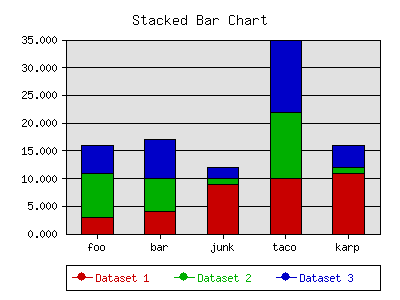
\includegraphics[scale=0.6]{stackedbars.png}
  \end{center}
  \caption{Chart with stacked bars}
  \label{fig:stackedbars}
\end{figure}
\begin{verbatim}
use Chart::StackedBars;

$g = Chart::StackedBars->new();

$g->add_dataset(qw(foo bar junk taco karp));
$g->add_dataset(3, 4, 9, 10, 11);
$g->add_dataset(8, 6, 1, 12, 1);
$g->add_dataset(5, 7, 2, 13, 4);

$g->set('title'        => 'Stacked Bar Chart');
$g->set('y_grid_lines' => 'true');
$g->set('legend'       => 'bottom');

$g->png("stackedbars.png");
\end{verbatim}

\constructorblurb{\thisname}

\begin{AttrDecl}{spaced\_bars}
Leaves some space between the individual bars when set to
\literal{true}. This usually make it easier to read a bar chart, with
stacked bars, however, it is not as important as with groups of bars.
Default is \literal{true}.
\end{AttrDecl}

\begin{AttrDecl}{y\_axes}
Tells \thisclass where to place the $y$ axis. Valid values are
\literal{left}, \literal{right} and \literal{both}. Defaults to
\literal{left}.
\end{AttrDecl}
